\section{Simulations}

Our experiments apply feedback alignment algorithm to network training on both synthetic and real-world data, where a range of networks with different activation functions and levels of regularization are considered. In particular, we compare the regularized feedback alignment (\cref{algo:fa-reg}) with its non-regularized counterpart (\cref{algo:fa}) on two-layer networks. We also evaluate the regularized feedback alignment algorithm with two-layer classification networks on \texttt{MNIST} dataset.

\paragraph{Synthetic dataset.}

For two-layer linear networks, the synthetic data for training are drawn from random linear models, where data $x_i$'s are independently generated and have independent standard Gaussian entries. The model parameter $\zeta\in\Rd$ is also independently generated with standard Gaussian entries, and the training label $y_i$ corresponding to $x_i$ is given by $y_i = x_i\transpose \zeta$. In our experiments, each time $n = 50$ data-label pairs $(x_i,y_i)$ are sampled from a random linear model with dimension $d = 150$, which forms one training dataset $(X,y)$ by stacking them as row vectors.

For two-layer non-linear networks, the generation process of training datasets is customized for different networks following the notion of a teacher-student model. If we deem the network to be trained as a student model, its training dataset is generated by a corresponding teacher model that is an independent and randomly initialized network of the same size and architecture. For each network $f$, its training data $x_i$'s are generated as independent Gaussian vectors like in the random linear model, and their corresponding labels are generated as the outputs of a two-layer network $y_i = f'(x_i)$, where $f'$ is an independent replica of $f$ with independent random Gaussian first- and second-layer weights. More specifically, if $f$ is a network with ReLU activation and hidden layer width $p$, then $f'$ is also a network with ReLU activation and hidden layer width $p$. In our experiments, all the training datasets $(X,y)$ consist of $n = 50$ training samples with dimension $d = 150$ and the training labels generated from an independent replica of the corresponding network.

\begin{figure}[h]
\centering

\begin{subfigure}[b]{.49\textwidth}
  \centering
  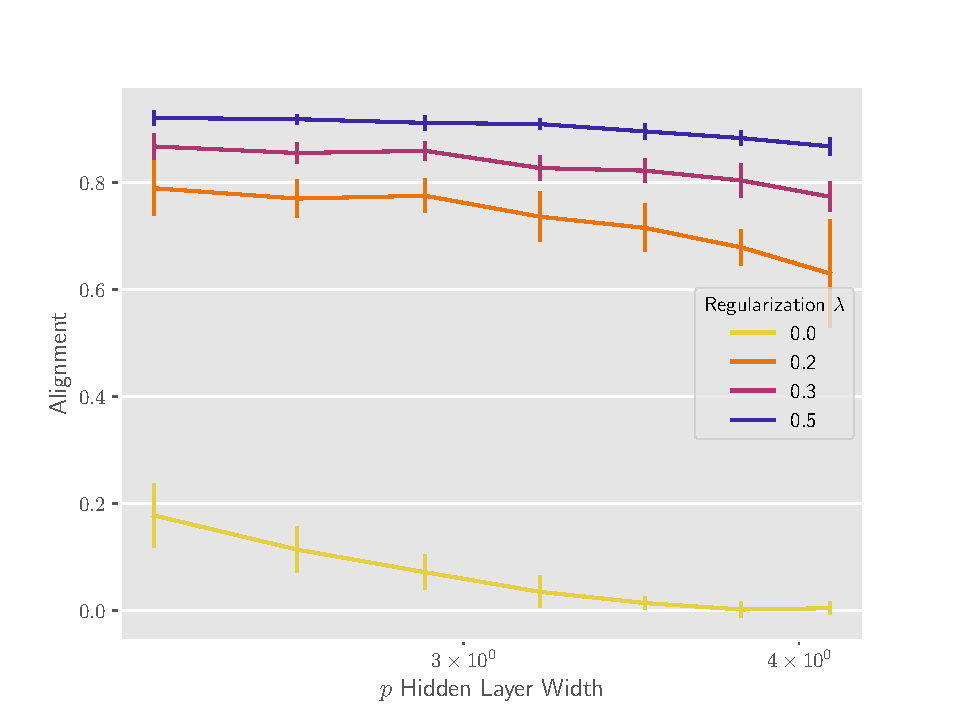
\includegraphics[width=\linewidth]{figures/align_lr_non_autograd_l2_v4.pdf}
  \caption{Alignment of linear network on linear regression data.}
  \label{fig:align_lr_non_autograd_l2}
\end{subfigure}\hfill
\begin{subfigure}[b]{.49\textwidth}
  \centering
  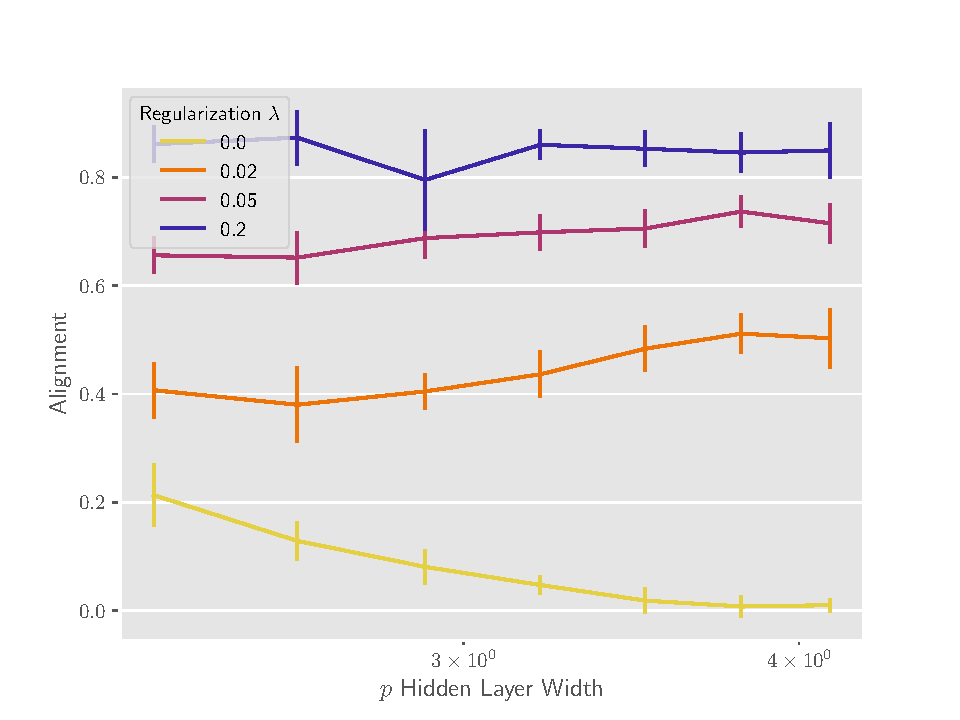
\includegraphics[width=\linewidth]{figures/align_nn_relu_autograd_l2_v4.pdf}
  \caption{Alignment of ReLU network on ReLU data.}
  \label{fig:align_nn_relu_autograd_l2}
\end{subfigure}

\medskip

\begin{subfigure}[b]{.49\textwidth}
  \centering
  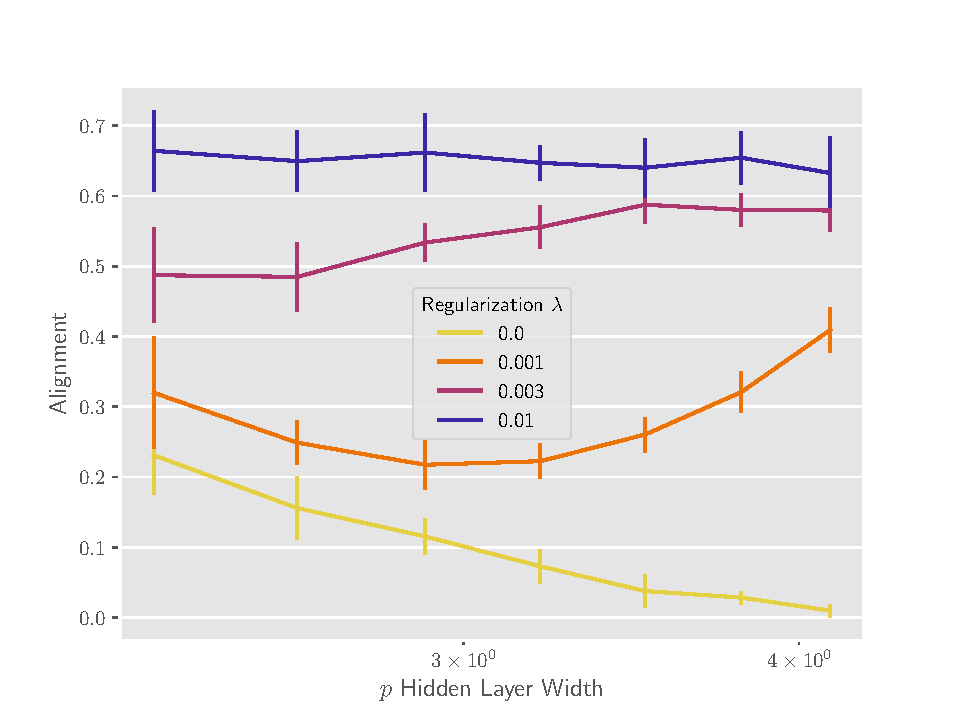
\includegraphics[width=\linewidth]{figures/align_nn_sigmoid_autograd_l2_v4.pdf}
  \caption{Alignment of Sigmoid network on Sigmoid data.}
  \label{fig:align_nn_sigmoid_autograd_l2}
\end{subfigure}\hfill
\begin{subfigure}[b]{.49\textwidth}
  \centering
  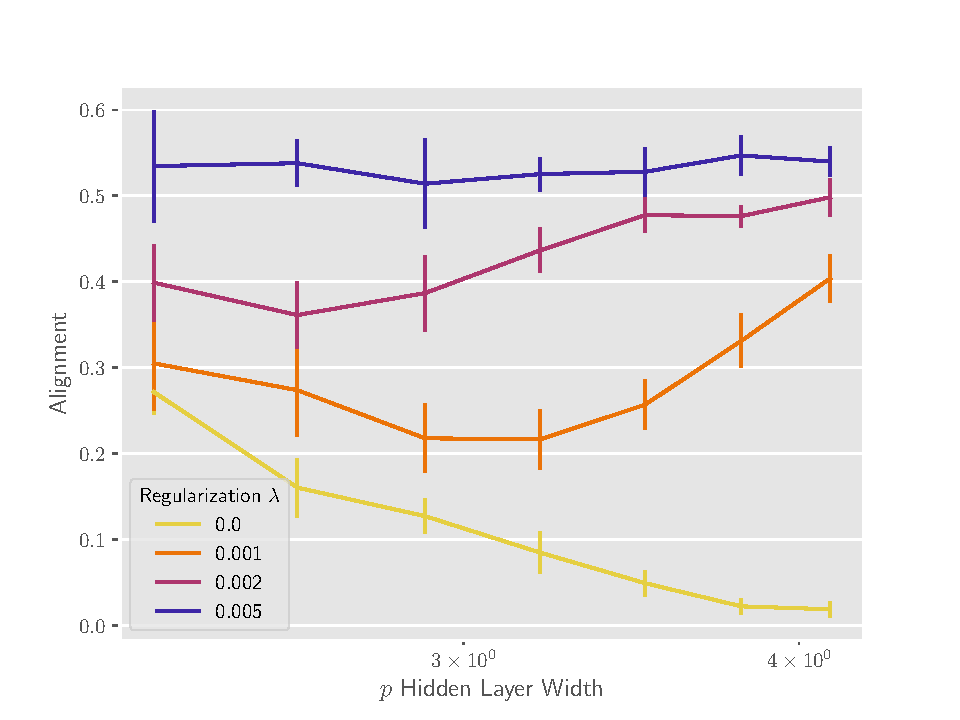
\includegraphics[width=\linewidth]{figures/align_nn_tanh_autograd_l2_v4.pdf}
  \caption{Alignment of Tanh network on Tanh data.}
  \label{fig:align_nn_tanh_autograd_l2}
\end{subfigure}
\caption{Synthetic data, l2. }
\label{fig:synthetic-l2}
\end{figure}

\paragraph{MNIST dataset.}

The training set of \texttt{MNIST} data consists of $6000$ black-and-white images of handwritten digits with dimension $28$ by $28$, and we flatten each of them into an one-dimensional vector of length $784$. The training data $x_i$'s are obtained after normalizing the vectors by their mean and standard deviation, and the test data can be similarly processed. We remark that the structure of the two-layer network we use for classification is slightly different from \cref{eqn:nonlinear-network}, 

\begin{figure}[t]
  \centering
  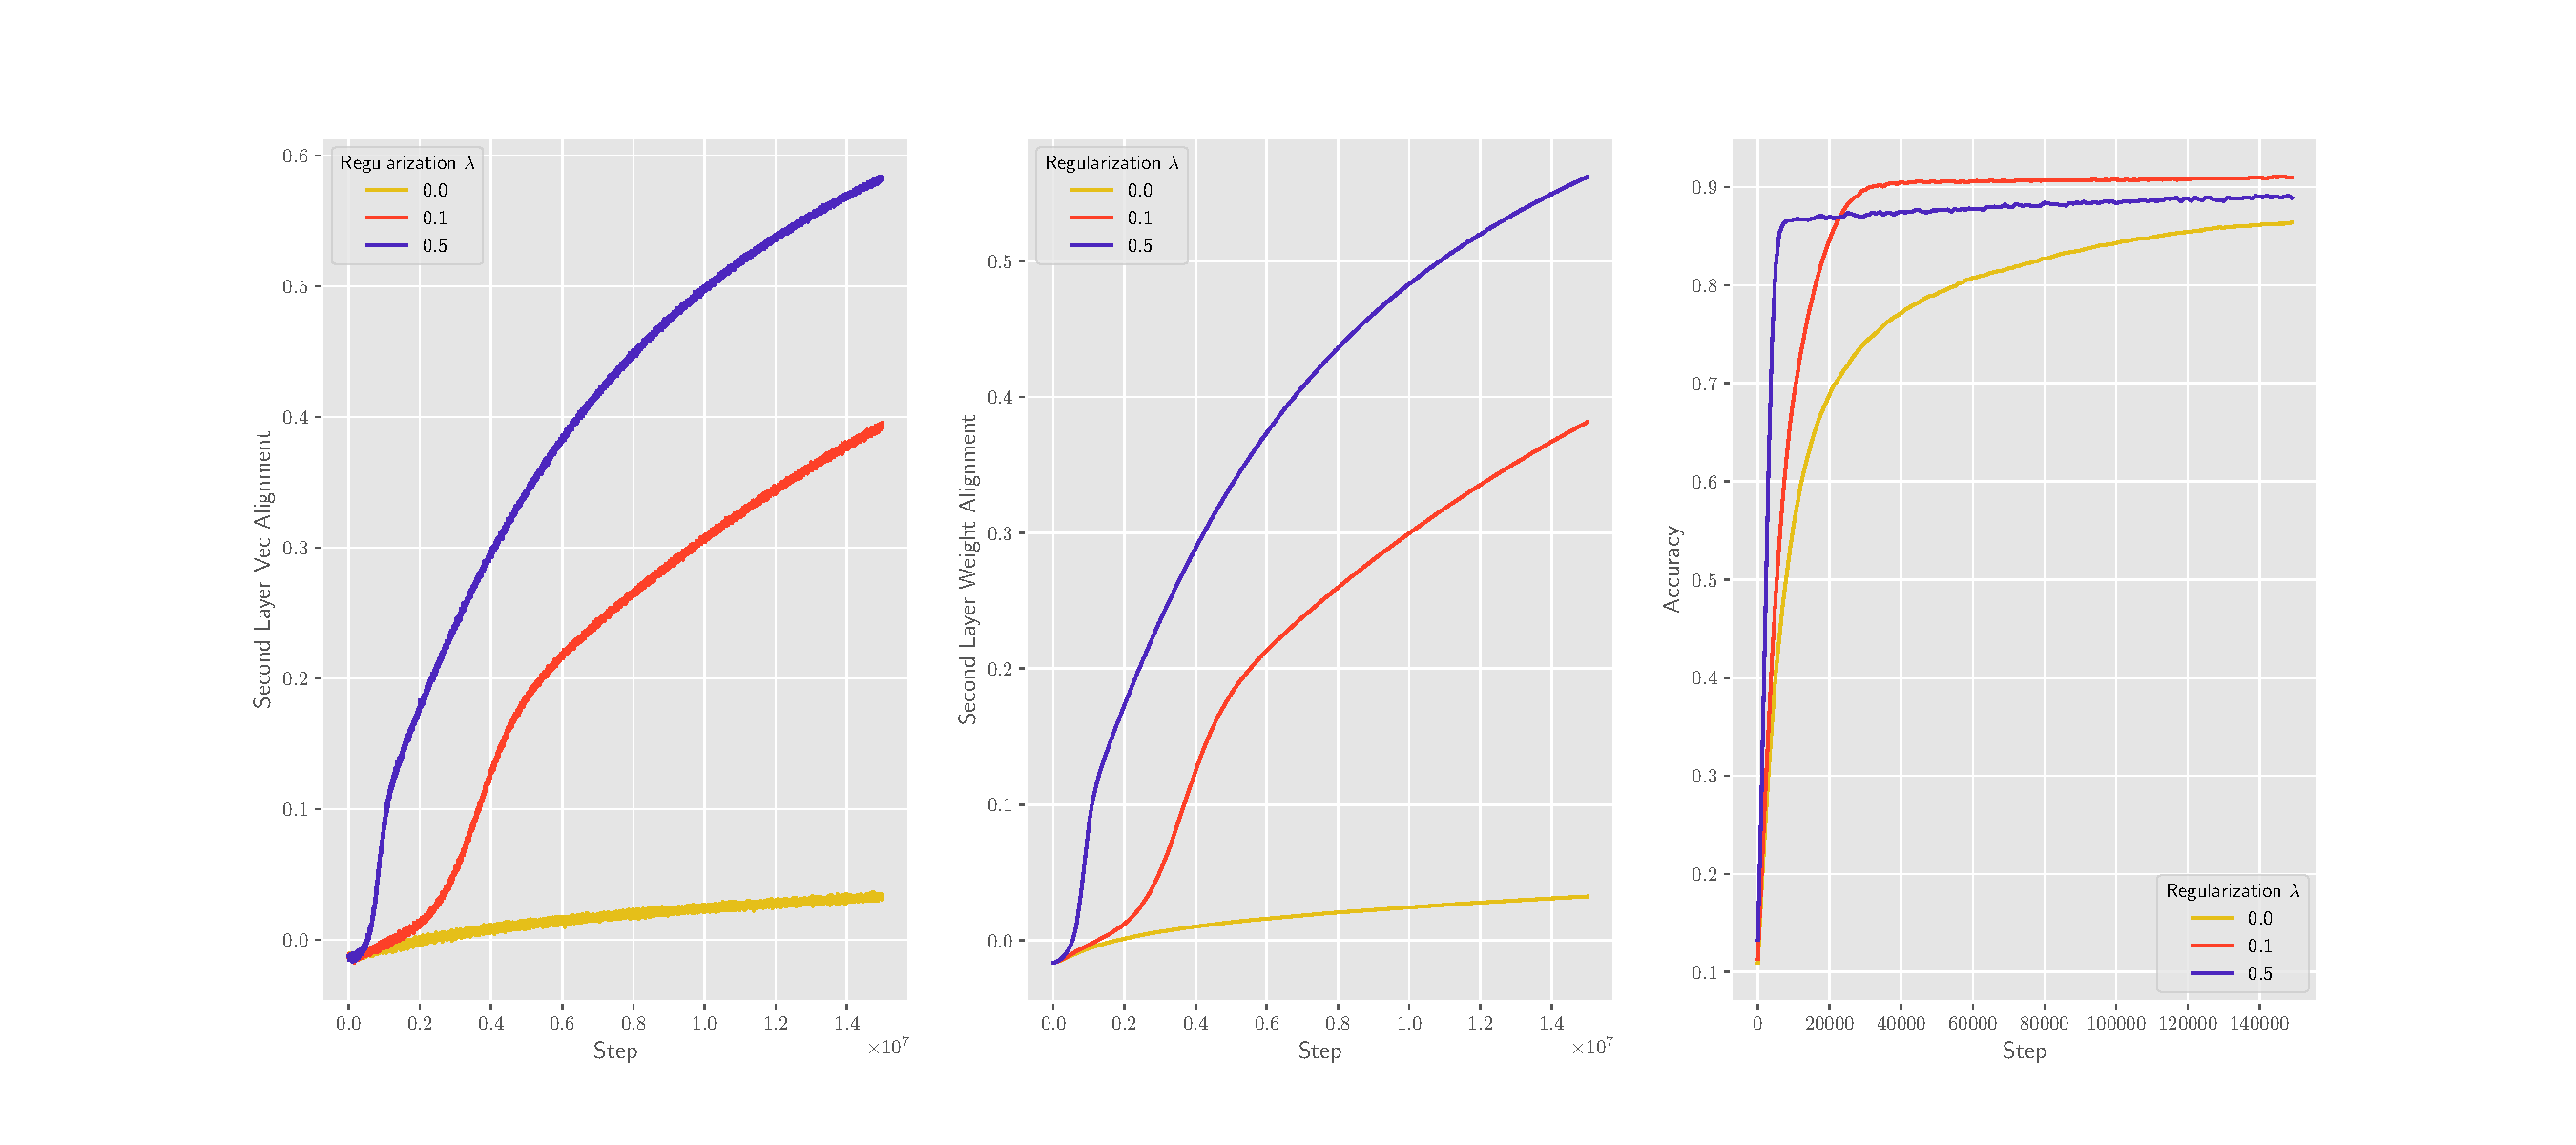
\includegraphics[width=\linewidth]{figures/mnist_2l_v2_horizontal.pdf}
  \caption{\texttt{MNIST} data.}
  \label{fig:mnist}
\end{figure}